\documentclass[9pt,t]{beamer}
% =====================================================================
% finance-beamer.tex — shared Beamer style for the LLM-in-Finance course
% =====================================================================
% Reusable slide style. Each deck \input's this immediately after
% \documentclass{beamer}. It provides:
%   * the Madrid theme + book colour palette (matches the printed book)
%   * two book-style framing blocks:
%       \begin{bigpicture} ... \end{bigpicture}   ("the bigger picture")
%       \begin{underhood}   ... \end{underhood}    ("under the hood")
%     These mirror the book's `context` and `deepdive` tcolorboxes so the
%     same intuition-vs-mechanism scaffold the reader meets in the book
%     reappears on the slides.
%   * a Python listings style for code frames
%   * appendix conventions: \appendixstart drops a divider and switches
%     to non-numbered backup frames so "extra / less central" material
%     lives after the main talk without inflating the slide count.
%
% Usage:
%   \documentclass{beamer}
%   % =====================================================================
% finance-beamer.tex — shared Beamer style for the LLM-in-Finance course
% =====================================================================
% Reusable slide style. Each deck \input's this immediately after
% \documentclass{beamer}. It provides:
%   * the Madrid theme + book colour palette (matches the printed book)
%   * two book-style framing blocks:
%       \begin{bigpicture} ... \end{bigpicture}   ("the bigger picture")
%       \begin{underhood}   ... \end{underhood}    ("under the hood")
%     These mirror the book's `context` and `deepdive` tcolorboxes so the
%     same intuition-vs-mechanism scaffold the reader meets in the book
%     reappears on the slides.
%   * a Python listings style for code frames
%   * appendix conventions: \appendixstart drops a divider and switches
%     to non-numbered backup frames so "extra / less central" material
%     lives after the main talk without inflating the slide count.
%
% Usage:
%   \documentclass{beamer}
%   % =====================================================================
% finance-beamer.tex — shared Beamer style for the LLM-in-Finance course
% =====================================================================
% Reusable slide style. Each deck \input's this immediately after
% \documentclass{beamer}. It provides:
%   * the Madrid theme + book colour palette (matches the printed book)
%   * two book-style framing blocks:
%       \begin{bigpicture} ... \end{bigpicture}   ("the bigger picture")
%       \begin{underhood}   ... \end{underhood}    ("under the hood")
%     These mirror the book's `context` and `deepdive` tcolorboxes so the
%     same intuition-vs-mechanism scaffold the reader meets in the book
%     reappears on the slides.
%   * a Python listings style for code frames
%   * appendix conventions: \appendixstart drops a divider and switches
%     to non-numbered backup frames so "extra / less central" material
%     lives after the main talk without inflating the slide count.
%
% Usage:
%   \documentclass{beamer}
%   \input{../_style/finance-beamer.tex}
%   \title{...}\subtitle{...}\author{...}\institute{...}\date{\today}
%   \begin{document} ... \end{document}
% =====================================================================

\usetheme{Madrid}
\usecolortheme{whale}
\setbeamertemplate{navigation symbols}{}
\setbeamertemplate{caption}[numbered]
\setbeamercovered{transparent}

% --- Density controls: keep dense, equation-heavy frames on one slide ---
% Slightly smaller body text + tighter lists/blocks. Frame titles and the
% Madrid chrome keep their normal size, so the deck still reads as Madrid,
% just with more vertical room for content.
\setbeamerfont{normal text}{size=\small}
\setbeamertemplate{itemize/enumerate body begin}{\small}
\setbeamertemplate{itemize/enumerate subbody begin}{\footnotesize}
% Tighter block spacing.
\setbeamertemplate{block begin}{%
  \par\vskip2pt%
  \begin{beamercolorbox}[colsep*=.75ex,leftskip=1ex,rightskip=1ex]{block title}%
    \usebeamerfont*{block title}\insertblocktitle%
  \end{beamercolorbox}%
  {\parskip0pt\vskip-1pt}%
  \begin{beamercolorbox}[colsep*=.75ex,vmode,leftskip=1ex,rightskip=1ex]{block body}%
  \vskip1pt}
\setbeamertemplate{block end}{\end{beamercolorbox}\vskip2pt}

\usepackage{amsmath, amssymb}
\usepackage{booktabs}
\usepackage{xcolor}
\usepackage{listings}
\usepackage[skins, breakable]{tcolorbox}

% --- Book colour palette (kept in sync with book/preamble.tex) ---
\definecolor{linkblue}{RGB}{14, 75, 140}
\definecolor{deepdivebg}{RGB}{235, 244, 255}
\definecolor{narrativebg}{RGB}{255, 252, 240}
\definecolor{narrativerule}{RGB}{180, 130, 40}
\definecolor{steelblue}{RGB}{70, 130, 180}
\definecolor{forestgreen}{RGB}{34, 139, 34}
\definecolor{crimson}{RGB}{220, 20, 60}
\definecolor{darkorange}{RGB}{255, 140, 0}
\definecolor{codebg}{RGB}{248, 248, 248}
\definecolor{coderule}{RGB}{210, 210, 210}
\definecolor{keywordblue}{RGB}{0, 100, 180}
\definecolor{commentgray}{RGB}{120, 120, 120}
\definecolor{stringgreen}{RGB}{30, 130, 30}

% Tie the Madrid structural colour to the book's link blue.
\setbeamercolor{structure}{fg=linkblue}
\setbeamercolor{title}{fg=white}
\setbeamercolor{frametitle}{fg=white}

% --- "the bigger picture" : narrative / intuition framing -----------
\newtcolorbox{bigpicture}{%
  enhanced, breakable, boxsep=2pt,
  colback  = narrativebg,
  colframe = narrativerule,
  boxrule  = 0pt, toprule = 1.4pt, bottomrule = 0.4pt,
  leftrule = 0pt, rightrule = 0pt, arc = 0pt,
  left = 6pt, right = 6pt, top = 4pt, bottom = 5pt,
  fonttitle = \footnotesize\scshape\color{narrativerule},
  title = {the bigger picture}, attach title to upper = {\par\smallskip},
}

% --- "under the hood" : the mechanism / technical detail ------------
\newtcolorbox{underhood}{%
  enhanced, breakable, boxsep=2pt,
  colback  = deepdivebg,
  colframe = linkblue,
  boxrule  = 0pt, toprule = 1.4pt, bottomrule = 0.4pt,
  leftrule = 0pt, rightrule = 0pt, arc = 0pt,
  left = 6pt, right = 6pt, top = 4pt, bottom = 5pt,
  fonttitle = \footnotesize\scshape\color{linkblue},
  title = {under the hood}, attach title to upper = {\par\smallskip},
}

% --- Python code style ---------------------------------------------
\lstset{
  basicstyle    = \ttfamily\footnotesize,
  keywordstyle  = \color{keywordblue}\bfseries,
  commentstyle  = \color{commentgray}\itshape,
  stringstyle   = \color{stringgreen},
  showstringspaces = false,
  language      = Python,
  breaklines    = true,
  backgroundcolor = \color{codebg},
  frame         = single,
  rulecolor     = \color{coderule},
  numbers       = none,
  aboveskip     = 4pt, belowskip = 4pt,
}

% --- Appendix conventions ------------------------------------------
% \appendixstart{Title} : begins the "extra material" appendix. Frames
% after it are not counted toward the main deck's frame total, keeping
% the core talk lean while preserving the deeper / optional content.
\newcommand{\appendixstart}[1]{%
  \appendix
  \setbeamertemplate{frametitle continuation}{}%
  \begin{frame}[noframenumbering]
    \begin{center}
      {\Large\scshape\color{linkblue} Appendix}\\[4pt]
      {\large #1}\\[10pt]
      {\footnotesize Extra / optional material — beyond the core lecture.}
    \end{center}
  \end{frame}
}
% Use \begin{frame}[noframenumbering]{...} for each appendix frame.

%   \title{...}\subtitle{...}\author{...}\institute{...}\date{\today}
%   \begin{document} ... \end{document}
% =====================================================================

\usetheme{Madrid}
\usecolortheme{whale}
\setbeamertemplate{navigation symbols}{}
\setbeamertemplate{caption}[numbered]
\setbeamercovered{transparent}

% --- Density controls: keep dense, equation-heavy frames on one slide ---
% Slightly smaller body text + tighter lists/blocks. Frame titles and the
% Madrid chrome keep their normal size, so the deck still reads as Madrid,
% just with more vertical room for content.
\setbeamerfont{normal text}{size=\small}
\setbeamertemplate{itemize/enumerate body begin}{\small}
\setbeamertemplate{itemize/enumerate subbody begin}{\footnotesize}
% Tighter block spacing.
\setbeamertemplate{block begin}{%
  \par\vskip2pt%
  \begin{beamercolorbox}[colsep*=.75ex,leftskip=1ex,rightskip=1ex]{block title}%
    \usebeamerfont*{block title}\insertblocktitle%
  \end{beamercolorbox}%
  {\parskip0pt\vskip-1pt}%
  \begin{beamercolorbox}[colsep*=.75ex,vmode,leftskip=1ex,rightskip=1ex]{block body}%
  \vskip1pt}
\setbeamertemplate{block end}{\end{beamercolorbox}\vskip2pt}

\usepackage{amsmath, amssymb}
\usepackage{booktabs}
\usepackage{xcolor}
\usepackage{listings}
\usepackage[skins, breakable]{tcolorbox}

% --- Book colour palette (kept in sync with book/preamble.tex) ---
\definecolor{linkblue}{RGB}{14, 75, 140}
\definecolor{deepdivebg}{RGB}{235, 244, 255}
\definecolor{narrativebg}{RGB}{255, 252, 240}
\definecolor{narrativerule}{RGB}{180, 130, 40}
\definecolor{steelblue}{RGB}{70, 130, 180}
\definecolor{forestgreen}{RGB}{34, 139, 34}
\definecolor{crimson}{RGB}{220, 20, 60}
\definecolor{darkorange}{RGB}{255, 140, 0}
\definecolor{codebg}{RGB}{248, 248, 248}
\definecolor{coderule}{RGB}{210, 210, 210}
\definecolor{keywordblue}{RGB}{0, 100, 180}
\definecolor{commentgray}{RGB}{120, 120, 120}
\definecolor{stringgreen}{RGB}{30, 130, 30}

% Tie the Madrid structural colour to the book's link blue.
\setbeamercolor{structure}{fg=linkblue}
\setbeamercolor{title}{fg=white}
\setbeamercolor{frametitle}{fg=white}

% --- "the bigger picture" : narrative / intuition framing -----------
\newtcolorbox{bigpicture}{%
  enhanced, breakable, boxsep=2pt,
  colback  = narrativebg,
  colframe = narrativerule,
  boxrule  = 0pt, toprule = 1.4pt, bottomrule = 0.4pt,
  leftrule = 0pt, rightrule = 0pt, arc = 0pt,
  left = 6pt, right = 6pt, top = 4pt, bottom = 5pt,
  fonttitle = \footnotesize\scshape\color{narrativerule},
  title = {the bigger picture}, attach title to upper = {\par\smallskip},
}

% --- "under the hood" : the mechanism / technical detail ------------
\newtcolorbox{underhood}{%
  enhanced, breakable, boxsep=2pt,
  colback  = deepdivebg,
  colframe = linkblue,
  boxrule  = 0pt, toprule = 1.4pt, bottomrule = 0.4pt,
  leftrule = 0pt, rightrule = 0pt, arc = 0pt,
  left = 6pt, right = 6pt, top = 4pt, bottom = 5pt,
  fonttitle = \footnotesize\scshape\color{linkblue},
  title = {under the hood}, attach title to upper = {\par\smallskip},
}

% --- Python code style ---------------------------------------------
\lstset{
  basicstyle    = \ttfamily\footnotesize,
  keywordstyle  = \color{keywordblue}\bfseries,
  commentstyle  = \color{commentgray}\itshape,
  stringstyle   = \color{stringgreen},
  showstringspaces = false,
  language      = Python,
  breaklines    = true,
  backgroundcolor = \color{codebg},
  frame         = single,
  rulecolor     = \color{coderule},
  numbers       = none,
  aboveskip     = 4pt, belowskip = 4pt,
}

% --- Appendix conventions ------------------------------------------
% \appendixstart{Title} : begins the "extra material" appendix. Frames
% after it are not counted toward the main deck's frame total, keeping
% the core talk lean while preserving the deeper / optional content.
\newcommand{\appendixstart}[1]{%
  \appendix
  \setbeamertemplate{frametitle continuation}{}%
  \begin{frame}[noframenumbering]
    \begin{center}
      {\Large\scshape\color{linkblue} Appendix}\\[4pt]
      {\large #1}\\[10pt]
      {\footnotesize Extra / optional material — beyond the core lecture.}
    \end{center}
  \end{frame}
}
% Use \begin{frame}[noframenumbering]{...} for each appendix frame.

%   \title{...}\subtitle{...}\author{...}\institute{...}\date{\today}
%   \begin{document} ... \end{document}
% =====================================================================

\usetheme{Madrid}
\usecolortheme{whale}
\setbeamertemplate{navigation symbols}{}
\setbeamertemplate{caption}[numbered]
\setbeamercovered{transparent}

% --- Density controls: keep dense, equation-heavy frames on one slide ---
% Slightly smaller body text + tighter lists/blocks. Frame titles and the
% Madrid chrome keep their normal size, so the deck still reads as Madrid,
% just with more vertical room for content.
\setbeamerfont{normal text}{size=\small}
\setbeamertemplate{itemize/enumerate body begin}{\small}
\setbeamertemplate{itemize/enumerate subbody begin}{\footnotesize}
% Tighter block spacing.
\setbeamertemplate{block begin}{%
  \par\vskip2pt%
  \begin{beamercolorbox}[colsep*=.75ex,leftskip=1ex,rightskip=1ex]{block title}%
    \usebeamerfont*{block title}\insertblocktitle%
  \end{beamercolorbox}%
  {\parskip0pt\vskip-1pt}%
  \begin{beamercolorbox}[colsep*=.75ex,vmode,leftskip=1ex,rightskip=1ex]{block body}%
  \vskip1pt}
\setbeamertemplate{block end}{\end{beamercolorbox}\vskip2pt}

\usepackage{amsmath, amssymb}
\usepackage{booktabs}
\usepackage{xcolor}
\usepackage{listings}
\usepackage[skins, breakable]{tcolorbox}

% --- Book colour palette (kept in sync with book/preamble.tex) ---
\definecolor{linkblue}{RGB}{14, 75, 140}
\definecolor{deepdivebg}{RGB}{235, 244, 255}
\definecolor{narrativebg}{RGB}{255, 252, 240}
\definecolor{narrativerule}{RGB}{180, 130, 40}
\definecolor{steelblue}{RGB}{70, 130, 180}
\definecolor{forestgreen}{RGB}{34, 139, 34}
\definecolor{crimson}{RGB}{220, 20, 60}
\definecolor{darkorange}{RGB}{255, 140, 0}
\definecolor{codebg}{RGB}{248, 248, 248}
\definecolor{coderule}{RGB}{210, 210, 210}
\definecolor{keywordblue}{RGB}{0, 100, 180}
\definecolor{commentgray}{RGB}{120, 120, 120}
\definecolor{stringgreen}{RGB}{30, 130, 30}

% Tie the Madrid structural colour to the book's link blue.
\setbeamercolor{structure}{fg=linkblue}
\setbeamercolor{title}{fg=white}
\setbeamercolor{frametitle}{fg=white}

% --- "the bigger picture" : narrative / intuition framing -----------
\newtcolorbox{bigpicture}{%
  enhanced, breakable, boxsep=2pt,
  colback  = narrativebg,
  colframe = narrativerule,
  boxrule  = 0pt, toprule = 1.4pt, bottomrule = 0.4pt,
  leftrule = 0pt, rightrule = 0pt, arc = 0pt,
  left = 6pt, right = 6pt, top = 4pt, bottom = 5pt,
  fonttitle = \footnotesize\scshape\color{narrativerule},
  title = {the bigger picture}, attach title to upper = {\par\smallskip},
}

% --- "under the hood" : the mechanism / technical detail ------------
\newtcolorbox{underhood}{%
  enhanced, breakable, boxsep=2pt,
  colback  = deepdivebg,
  colframe = linkblue,
  boxrule  = 0pt, toprule = 1.4pt, bottomrule = 0.4pt,
  leftrule = 0pt, rightrule = 0pt, arc = 0pt,
  left = 6pt, right = 6pt, top = 4pt, bottom = 5pt,
  fonttitle = \footnotesize\scshape\color{linkblue},
  title = {under the hood}, attach title to upper = {\par\smallskip},
}

% --- Python code style ---------------------------------------------
\lstset{
  basicstyle    = \ttfamily\footnotesize,
  keywordstyle  = \color{keywordblue}\bfseries,
  commentstyle  = \color{commentgray}\itshape,
  stringstyle   = \color{stringgreen},
  showstringspaces = false,
  language      = Python,
  breaklines    = true,
  backgroundcolor = \color{codebg},
  frame         = single,
  rulecolor     = \color{coderule},
  numbers       = none,
  aboveskip     = 4pt, belowskip = 4pt,
}

% --- Appendix conventions ------------------------------------------
% \appendixstart{Title} : begins the "extra material" appendix. Frames
% after it are not counted toward the main deck's frame total, keeping
% the core talk lean while preserving the deeper / optional content.
\newcommand{\appendixstart}[1]{%
  \appendix
  \setbeamertemplate{frametitle continuation}{}%
  \begin{frame}[noframenumbering]
    \begin{center}
      {\Large\scshape\color{linkblue} Appendix}\\[4pt]
      {\large #1}\\[10pt]
      {\footnotesize Extra / optional material — beyond the core lecture.}
    \end{center}
  \end{frame}
}
% Use \begin{frame}[noframenumbering]{...} for each appendix frame.


\title{Explainability and Interpretability of LLMs in Finance}
\subtitle{Lecture 12 --- Explainable AI for Finance}
\author{Juan F.\ Imbet}
\institute{Paris Dauphine -- PSL University}
\date{\today}

\begin{document}

% ============================================================
\begin{frame}\titlepage\end{frame}

\begin{frame}{Outline}\tableofcontents\end{frame}

% ============================================================
\section{Why Explainability Matters in Regulated Finance}
% ============================================================

% --- Frame: the loan-rejection scenario ---
\begin{frame}{The Problem in One Scenario}
\begin{bigpicture}
A small-business owner applies for a working-capital loan. A transformer-based
credit system returns a \emph{rejection} in seconds. Under the Equal Credit
Opportunity Act, the loan officer must give the applicant \textbf{specific
reasons}. The model offers only a probability --- not a rationale.
\end{bigpicture}

\medskip
\textbf{Explainability} = the degree to which a human can understand the cause
of a model's decision (Miller, 2019).

\medskip
\begin{block}{Why finance is different}
In most industries opacity is an inconvenience. In finance it is a
\textbf{legal, fiduciary, and reputational} problem. Institutions must show
that outputs are \emph{appropriate, non-discriminatory, and auditable} --- not
merely accurate (SR 11-7).
\end{block}

\medskip
\textbf{LLMs sharpen the challenge:} billions of parameters, uninterpretable
activations, and outputs that depend on prompt phrasing in ways that are hard
to characterise.
\end{frame}

% --- Frame: legal requirements ---
\begin{frame}{Legal Requirements: Four Frameworks}
\small
\begin{tabular}{p{2.1cm}p{8.0cm}}
\toprule
\textbf{Framework} & \textbf{What it demands} \\
\midrule
EU AI Act (2024) & Credit scoring / insurance pricing = \emph{high-risk}
  (Annex III). Transparency, input/output logging, human oversight; must
  explain what drove a \emph{specific} decision. \\[2pt]
SR 11-7 (Fed) & Model-risk management: document conceptual soundness; outputs
  explainable to non-technical risk managers; sensitivity \& post-hoc
  attribution. \\[2pt]
ECOA / Reg.\ B & Adverse-action notices must give the ``principal reasons''
  (4--5 factors) in plain language. ``Not creditworthy'' is \emph{not} enough. \\[2pt]
GDPR Art.\ 22 / FCRA & Right to a ``meaningful explanation'' of the logic of
  solely-automated decisions. \\
\bottomrule
\end{tabular}

\medskip
\begin{alertblock}{Definition --- Explanation vs.\ Interpretation}
\textbf{Interpretation:} how does the model work \emph{in general}?
\textbf{Explanation:} why this output for \emph{this} input?
Regulation is primarily \textbf{explanatory} --- specific decisions justified to
specific persons (Doshi-Velez \& Kim, 2017).
\end{alertblock}
\end{frame}

% --- Frame: stakeholders ---
\begin{frame}{Three Audiences, Three Tolerances}
\begin{columns}[T]
\begin{column}{0.5\textwidth}
\textbf{Clients / applicants}
\begin{itemize}\small
  \item Actionable, plain-language, contrastive
  \item ``DTI of 52\% was 10 pp above threshold'' \\
        $\succ$ ``$x_{17}$ had SHAP $-0.43$''
\end{itemize}
\medskip
\textbf{Regulators / examiners}
\begin{itemize}\small
  \item Higher technical rigour
  \item Global behaviour: disparate impact?
  \item Audit any case on complaint
\end{itemize}
\end{column}
\begin{column}{0.5\textwidth}
\textbf{Auditors / validators}
\begin{itemize}\small
  \item Both global + local
  \item Must \textbf{reproduce} explanations
  \item Non-deterministic XAI is unfit for audit
\end{itemize}
\end{column}
\end{columns}

\medskip
\begin{block}{Design tension}
Methods that satisfy regulators may overwhelm retail clients; methods accessible
to clients may be too simplified for auditors. A real strategy deploys
\textbf{multiple explanation types in parallel}.
\end{block}
\end{frame}

% --- Frame: black box problem ---
\begin{frame}{The Black-Box Problem for LLMs}
\textbf{Intrinsically interpretable} classics:
\begin{itemize}
  \item Logistic regression: score = weighted sum; weights \emph{are} the interpretation.
  \item Decision tree: a readable set of binary-split rules.
\end{itemize}

\medskip
\textbf{LLMs are not} interpretable in this sense:
\begin{itemize}
  \item Knowledge in \emph{distributed} representations across all layers --- no
        parameter maps to a human concept.
  \item Attention $\ne$ causal explanation (later).
  \item Inputs can be \emph{free text} $\Rightarrow$ effectively infinite input
        space $\Rightarrow$ exhaustive sensitivity analysis impossible.
\end{itemize}

\medskip
\begin{alertblock}{Rudin (2019): stop explaining black boxes}
For high-stakes decisions, prefer \emph{intrinsically interpretable} models.
\textbf{Rejoinder for finance:} a model that jointly reads financial ratios
\emph{and} qualitative business text may extract signal a numeric model cannot.
Whether the extra signal is worth the interpretability cost is a
\emph{business/regulatory} judgement, not a technical one.
\end{alertblock}
\end{frame}

% ============================================================
\section{Classical XAI Methods Applied to LLMs}
% ============================================================

% --- Frame: SHAP from game theory ---
\begin{frame}{SHAP: Shapley Values from Cooperative Game Theory}
\begin{bigpicture}
Treat each \emph{feature} as a \emph{player} in a cooperative game. A feature's
attribution is its average marginal contribution across all orderings in which
players join the coalition --- a provably ``fair'' division of the prediction.
\end{bigpicture}

\begin{underhood}
For a game $(N,v)$ with $v(\emptyset)=0$, the Shapley value of player $i$ is
\[
\phi_i(v) = \sum_{S \subseteq N \setminus \{i\}}
\frac{|S|!\,(n-|S|-1)!}{n!}\bigl[v(S \cup \{i\}) - v(S)\bigr].
\]
\textbf{SHAP} (Lundberg \& Lee, 2017): players $=$ features $x_1,\dots,x_n$;
$v(S)=$ expected prediction with only $S$ ``known''. Then $\phi_i$ is how much
feature $i$ moves the prediction from the baseline $\mathbb{E}[f(X)]$.
\end{underhood}
\end{frame}

% --- Frame: SHAP properties (continued) ---
\begin{frame}{SHAP: Three Properties Prized in Finance}
The Shapley division is not just convenient --- it is the \emph{unique}
attribution satisfying a set of axioms. Three of them matter directly for
regulated credit work:
\begin{itemize}
  \item \textbf{Efficiency:} $\sum_i \phi_i = f(x) - \mathbb{E}[f(X)]$ (accounts
        for the whole prediction).
  \item \textbf{Symmetry:} identical contributions $\Rightarrow$ equal values.
  \item \textbf{Dummy:} irrelevant features get zero.
\end{itemize}

\medskip
\begin{block}{Why this matters for ECOA}
Efficiency guarantees the attributions \emph{add up} to the decision: no part of
the rejection is left unexplained. Symmetry and dummy give the fairness footing ---
features are treated consistently and irrelevant ones cannot be blamed.
\end{block}
\end{frame}

% --- Frame: SHAP for LLMs + credit example ---
\begin{frame}{SHAP for LLMs: A Credit-Decision Example}
\textbf{What is a ``feature'' in text?} The \textbf{token}. But marginalising a
token requires a reference: a mask token, a random vocabulary token, or sampling
from a small reference LM. TreeSHAP is exact in poly-time; for LLMs we
\emph{approximate} (KernelSHAP).

\medskip
\begin{columns}[T]
\begin{column}{0.52\textwidth}
\footnotesize
Fine-tuned BERT $\to$ $P(\text{creditworthy})=0.14$ (baseline $0.50$).
KernelSHAP, 500 samples:
\begin{tabular}{lr}
\toprule
Token & SHAP \\
\midrule
struggled   & $-0.089$ \\
declining   & $-0.073$ \\
down 30\%   & $-0.061$ \\
competitive & $-0.047$ \\
restaurant  & $-0.038$ \\
pandemic    & $-0.029$ \\
operates    & $+0.012$ \\
\bottomrule
\end{tabular}
\end{column}
\begin{column}{0.48\textwidth}
\footnotesize
Negative tokens cover most of the $0.50 - 0.14 = 0.36$ gap.

\medskip
$\Rightarrow$ partial ECOA statement: ``primarily affected by language indicating
declining revenue, operational struggle, and market difficulties.''

\medskip
\begin{alertblock}{Caveat}
SHAP measures \emph{correlational} importance \emph{within the model} --- not
real-world causation. A spurious correlation (jargon $\leftrightarrow$
protected class) is reported faithfully. Fairness auditing is a
\textbf{separate} step.
\end{alertblock}
\end{column}
\end{columns}
\end{frame}

% --- Frame: LIME ---
\begin{frame}{LIME: Local, Model-Agnostic Surrogates}
\begin{bigpicture}
A globally non-linear model is \emph{locally} approximately linear. Fit a sparse
interpretable model in the neighbourhood of the instance being explained.
\end{bigpicture}

\textbf{Recipe:} (1) perturb $x$ by masking features $\to z_1,\dots,z_K$;
(2) query $f(z_k)$; (3) fit sparse linear $g$ weighted by proximity
$\pi_x(z)=\exp(-D(x,z)^2/\sigma^2)$.

\begin{underhood}
\[
\xi(x) = \arg\min_{g \in \mathcal{G}}\;
\underbrace{\textstyle\sum_k \pi_x(z_k)\bigl(f(z_k)-g(z_k)\bigr)^2}_{\mathcal{L}:\;\text{locality-weighted fidelity}}
\;+\;\underbrace{\Omega(g)}_{\text{complexity}}.
\]
\end{underhood}

\medskip
\begin{columns}[T]
\begin{column}{0.5\textwidth}
\textbf{Advantage:} truly model-agnostic --- only needs query access. Works on
closed APIs (GPT-4, Claude) with \emph{no} gradients.
\end{column}
\begin{column}{0.5\textwidth}
\textbf{Disadvantage:} \emph{instability} --- stochastic perturbations $\Rightarrow$
different explanations on reruns. \textbf{Fix a seed} for audit reproducibility.
\end{column}
\end{columns}
\end{frame}

% --- Frame: attention as explanation ---
\begin{frame}{Attention Visualisation: Promise and Limits}
Attention weight $\alpha_{ij}=\operatorname{softmax}(\mathbf{Q}\mathbf{K}^\top/\sqrt{d_k})_{ij}$
normalises to one $\Rightarrow$ \emph{tempting} to read as ``token $j$ drove the
output.'' Practitioners colour tokens by $\alpha$.

\medskip
\begin{alertblock}{Why this is weak}
\textbf{Jain \& Wallace (2019):} adversarial \emph{alternative} attention
distributions give \emph{identical} predictions $\Rightarrow$ attention is not a
unique explanation. \textbf{Wiegreffe \& Pinter (2019):} attention can still be a
useful \emph{diagnostic}, not a causal account.
\end{alertblock}

\begin{block}{Definition --- Faithfulness vs.\ Plausibility (Jacovi \& Goldberg, 2020)}
\textbf{Faithful:} accurately reflects the causal process producing the output.
\textbf{Plausible:} looks convincing to humans, regardless of the true computation.
\end{block}

\medskip
Attention is often \emph{plausible} but \emph{unfaithful} --- dangerous: it can
make an auditor certify a decision as well-reasoned when the real drivers differ.
\textbf{Integrated Gradients} (Sundararajan, 2017) gives stronger faithfulness
(needs gradients $\Rightarrow$ no closed APIs).
\end{frame}

% ============================================================
\section{LLM-Native Explainability Mechanisms}
% ============================================================

% --- Frame: chain of thought ---
\begin{frame}{Chain-of-Thought as an Explanation Trace}
\begin{bigpicture}
Instead of black-box post-hoc methods, exploit the LLM's own generation: have it
emit a reasoning trace \emph{before} the answer. The trace doubles as a
plain-language explanation regulators can read and archive.
\end{bigpicture}

\textbf{Dual function of CoT (Wei et al., 2022):}
\begin{enumerate}\small
  \item Improves decision quality on multi-step inference (e.g.\ covenant-breach checks).
  \item The trace is a natural-language explanation for applicant + auditor.
\end{enumerate}

\begin{underhood}
\textbf{Definition --- Explanation Trace.} A sequence $r_1,\dots,r_T$ generated
before output $\hat{y}$, each $r_t$ following from prior steps and input $x$,
together entailing $\hat{y}$. \emph{Counterfactually faithful} if negating any
$r_t$ flips $\hat{y}$.
\end{underhood}
\end{frame}

% --- Frame: chain of thought (faithfulness risk) ---
\begin{frame}{Chain-of-Thought: The Faithfulness Risk}
A reasoning trace \emph{looks} like an explanation. The danger is treating it as
one without evidence that it reflects how the model actually decided.

\medskip
\begin{alertblock}{Faithfulness risk}
The model's real inference is parallel matrix computation --- not sequential
reasoning. A fluent trace may not reflect it. \textbf{Self-consistency} (Wang et
al., 2022): sample $K$ traces, take the majority answer $\Rightarrow$ more
accurate, more consistent.
\end{alertblock}

\medskip
\begin{block}{Practical stance for finance}
Use CoT for its \emph{decision-quality} gains and as a \emph{human-readable}
draft, but do not present the trace to a regulator as the causal account of the
decision unless it has passed a counterfactual-faithfulness check.
\end{block}
\end{frame}

% --- Frame: counterfactuals ---
\begin{frame}{Counterfactual Explanations: What Would Change It?}
Different question: not ``what drove the decision?'' but ``what is the closest
state of affairs in which it flips?'' \textbf{Actionable by construction}
(Wachter et al., 2017).

\medskip
``DTI of 54\% was a key negative'' \quad$\prec$\quad ``a ratio below 45\% would
likely lead to approval, all else equal.''

\begin{underhood}
\[
x' = \arg\min_{z \in \mathcal{X}} d(x,z)\quad\text{s.t.}\quad f(z)=c,\quad c \ne f(x),
\]
with $d$ a cost-reflecting distance: weighted $\ell_1/\ell_2$ for structured
inputs, edit / token-substitution distance for text.
\end{underhood}
\end{frame}

% --- Frame: counterfactuals (feasibility) ---
\begin{frame}{Counterfactuals: Feasibility and Legality Constraints}
Solving the optimisation is only half the job. The \emph{closest} counterfactual
is often not one a person can act on --- or one a lender may legally cite.

\medskip
\begin{block}{Text makes this hard --- and constraints matter}
Discrete input space $\Rightarrow$ no direct gradient descent. Two-stage:
identify sensitive dimensions, then articulate them (often \emph{with} an LLM).
The closest counterfactual may be \textbf{infeasible} (``if your age were
different'') or \textbf{illegal} --- age is protected under ECOA. Add feasibility
\& non-discrimination constraints.
\end{block}

\medskip
\begin{alertblock}{The actionability payoff}
Done right, a counterfactual turns a denial into guidance: ``lower your DTI below
45\%'' is something an applicant can pursue, unlike a raw SHAP score. That is why
it is the explanation form regulators and clients both tend to prefer.
\end{alertblock}
\end{frame}

% --- Frame: NL justifications ---
\begin{frame}{Natural-Language Justifications: Separation of Concerns}
\textbf{Pipeline:} (1) a primary model decides; (2) SHAP / IG identifies top
drivers; (3) an LLM \emph{translates} those drivers into plain-language prose for
the target audience.

\medskip
\begin{block}{Why separate the three roles}
\begin{tabular}{ll}
Primary model & evaluated for \emph{predictive accuracy} \\
Attribution & evaluated for \emph{faithfulness} to that model \\
LLM generator & evaluated for \emph{clarity, completeness, compliance} \\
\end{tabular}
Each component is independently testable and replaceable.
\end{block}

\medskip
\begin{alertblock}{The generator must not hallucinate attributions}
If SHAP said ``revenue decline,'' the generator must \emph{not} add ``poor
personal credit history'' --- even if plausible. Feed attribution scores as
\textbf{structured input}; constrain via prompt engineering or constrained
decoding to refer \emph{only} to provided attributions.
\end{alertblock}
\end{frame}

% ============================================================
\section{Case Studies in Financial Explainability}
% ============================================================

% --- Frame: hybrid credit pipeline ---
\begin{frame}[fragile]{Case Study 1: Hybrid SME Credit-Scoring Pipeline}
A fintech lender's three-stage pipeline:
\begin{enumerate}\small
  \item \textbf{Structured (42 vars):} gradient-boosted tree $+$ \emph{exact} TreeSHAP.
  \item \textbf{Unstructured text:} fine-tuned DistilBERT $+$ KernelSHAP (1{,}000 samples) $\to$ top-5 negative tokens.
  \item \textbf{Adverse-action generation:} GPT-4o, constrained to the feed below.
\end{enumerate}

\begin{lstlisting}[language=]
You are a credit officer drafting a regulatory-compliant
adverse action notice. The application was declined. The
primary reasons, in order of importance, are:
1. Debt-to-income ratio: 54% (threshold 45%)  - SHAP -0.18
2. Revenue trend: -28% YoY                     - SHAP -0.12
3. Description: "struggling","declining"       - txt  -0.09
4. Cash reserve: 0.8 mo (threshold 3)          - SHAP -0.07
5. Industry: Hospitality (elevated default)    - SHAP -0.05
Do NOT introduce factors not listed. Do NOT mention protected
characteristics. Limit to 150 words.
\end{lstlisting}

\textbf{Principle:} LLMs are safest in the explanation layer when inputs are
\emph{tightly constrained by upstream attribution}. The LLM transforms
attributions into prose; it must not exercise credit judgement here.
\end{frame}

% --- Frame: ECOA/FCRA letters ---
\begin{frame}{Case Study 2: ECOA/FCRA-Compliant Denial Letters}
Reg.\ B requires notice within \textbf{30 days}: (1) specific reasons,
(2) right to a statement of reasons, (3) right to a free consumer-report copy if
used. ``Principal reasons'' = typically 4--5, stated \emph{specifically}.

\medskip
\begin{columns}[T]
\begin{column}{0.5\textwidth}
\begin{alertblock}{Failure mode 1: vagueness}
``credit profile did not meet criteria'' --- insufficient.\\
``DTI 54\% exceeded our 45\% max'' --- compliant.
\end{alertblock}
\end{column}
\begin{column}{0.5\textwidth}
\begin{alertblock}{Failure mode 2: protected factors}
Demographic signals in text $\Rightarrow$ explanation may reference race,
sex, age\ldots\ Must filter.
\end{alertblock}
\end{column}
\end{columns}

\medskip
\textbf{Robust implementation:}
\begin{enumerate}\small
  \item Structured attribution feed --- \emph{non-protected} variables only.
  \item System prompt forbidding new factors / protected characteristics.
  \item Post-generation compliance check (classifier / keyword filter).
  \item Human-review queue for any flagged letter.
\end{enumerate}
\end{frame}

% --- Frame: MiFID II ---
\begin{frame}{Case Study 3: MiFID II Suitability Disclosures}
MiFID II: investment firms must give retail clients a \textbf{suitability
report} explaining why a product fits their objectives, risk tolerance,
situation, and knowledge --- \emph{before} execution.

\medskip
\textbf{CFA Institute (2025) --- three requirements for AI-generated disclosures:}
\begin{enumerate}\small
  \item Reasoning \textbf{traceable} to the client data on file.
  \item Language must \textbf{not} overstate returns or understate risks.
  \item \textbf{Auditable / reproducible}: same data + config $\to$ materially
        equivalent document.
\end{enumerate}

\medskip
\begin{exampleblock}{Robo-adviser, $n=12{,}000$ clients, annual review}
Structured profile $\to$ risk tier + suitability score $\to$ Integrated Gradients
$\to$ top-3 drivers $\to$ LLM prompted to use stated horizon \& risk tolerance,
acknowledge capital-loss risk, cite no return figure absent from the KID $\to$
compliance filter. \textbf{Quarterly 2\% human sample}; illustrative revision
rate $\approx 0.3\%$, all from objective-vs-product tension.
\end{exampleblock}
\end{frame}

% ============================================================
\section{Evaluating the Quality of Explanations}
% ============================================================

% --- Frame: faithfulness metrics ---
\begin{frame}{Faithfulness: Sufficiency and Comprehensiveness}
\textbf{The hard part:} unlike predictions, there is \emph{no ground-truth
explanation} to benchmark against.

\begin{underhood}
Let $e(x)$ be the explained (important) features, $\bar{e}(x)$ its complement.
\begin{align*}
\text{Suff}(e,f,x) &= 1 - |f(x) - f(x_{e(x)})|
  &&\text{(keep only }e\text{: prediction preserved?)}\\
\text{Comp}(e,f,x) &= |f(x) - f(x_{\bar{e}(x)})|
  &&\text{(remove }e\text{: prediction degraded?)}
\end{align*}
Suff $\to 1$ = perfect faithfulness; high Comp = the explained features really drove it.
\end{underhood}

\medskip
\begin{block}{How the methods score}
\begin{tabular}{ll}
SHAP & efficiency property $\Rightarrow$ a form of \emph{sufficiency} for the full set \\
LIME & may \emph{fail} sufficiency: deliberately sparse surrogate omits correlated features \\
Attention & typically \emph{fails comprehensiveness}: ablating attended tokens often
  leaves output unchanged
\end{tabular}
\end{block}
\end{frame}

% --- Frame: completeness + plausibility ---
\begin{frame}{Completeness and Plausibility}
\begin{columns}[T]
\begin{column}{0.5\textwidth}
\textbf{Completeness}\\
Does it account for \emph{all} relevant drivers, not just the top one? An ECOA
notice citing 1 of 5 significant reasons is incomplete.

\medskip
For SHAP, directly measurable:
\[
\frac{\sum_{i \in e(x)} \phi_i}{f(x) - \mathbb{E}[f(X)]}.
\]
\end{column}
\begin{column}{0.5\textwidth}
\textbf{Plausibility}\\
Would a domain expert agree it makes sense?
``high DTI'' = plausible; ``the word \emph{the}'' = implausible (even if accurate).

\medskip
Correlates with --- but is \emph{not} --- faithfulness. Measured by agreement with
expert-annotated ground truth, or readability for ECOA audiences.
\end{column}
\end{columns}

\medskip
\begin{alertblock}{Key distinction}
A plausible explanation may be faithful \emph{or} unfaithful. Plausibility alone
is a poor quality gate.
\end{alertblock}
\end{frame}

% --- Frame: human subject studies ---
\begin{frame}{Human-Subject Studies with Domain Experts}
The ultimate regulatory test: can a qualified expert \emph{use} the explanation
to make appropriate decisions? Three standard designs (Doshi-Velez \& Kim, 2017):

\medskip
\begin{tabular}{p{3.0cm}p{7.2cm}}
\toprule
\textbf{Forward simulation} & Given an explanation, predict the model's output on
  a held-out input. \\[2pt]
\textbf{Decision support} & Approve/reject with vs.\ without explanations ---
  does it help catch model errors? \\[2pt]
\textbf{Trust calibration} & Should \emph{raise} trust on correct predictions,
  \emph{lower} it on incorrect ones. \\
\bottomrule
\end{tabular}

\medskip
\textbf{Practical constraint:} credit officers / compliance specialists are
expensive participants. Alternative: \emph{vignette studies} with synthetic
scenarios via professional networks.

\medskip
\begin{alertblock}{The trap}
Experts often find plausible-but-unfaithful explanations \emph{just as
satisfying} as faithful ones. Human evaluation alone is not a reliable gate ---
pair it with quantitative faithfulness metrics.
\end{alertblock}
\end{frame}

% ============================================================
\section{Summary}
% ============================================================

\begin{frame}{Five Takeaways}
\begin{enumerate}
  \item \textbf{Explainability is a legal requirement}, not an aspiration:
        EU AI Act, SR 11-7, ECOA, MiFID II.
  \item \textbf{Classical XAI adapts to LLMs but not trivially}: SHAP \& LIME
        need feature definitions + marginalisation/perturbation schemes; both can
        be unstable.
  \item \textbf{Attention is not faithful} in general; gradient methods
        (Integrated Gradients) are stronger but need model internals.
  \item \textbf{LLM-native methods} (CoT, counterfactuals, NL justifications) give
        plain language --- but constrain the generator to upstream attributions
        and add compliance filters.
  \item \textbf{Evaluate on multiple axes:} faithfulness, completeness,
        plausibility, human utility. No single metric suffices.
\end{enumerate}

\medskip
\begin{block}{The recurring architecture}
Decide $\to$ attribute (faithfully) $\to$ translate (constrained LLM) $\to$ filter
(compliance) $\to$ human review. Auditable at every stage.
\end{block}
\end{frame}

% ============================================================
% APPENDIX
% ============================================================
\appendixstart{Deeper Foundations, Benchmarks \& Further Reading}

% --- Appendix: Shapley properties / TreeSHAP ---
\begin{frame}[noframenumbering]{Appendix A: Why Shapley Values Are ``Fair''}
The combinatorial weight $\dfrac{|S|!\,(n-|S|-1)!}{n!}$ is the probability that
feature $i$ joins coalition $S$ at this position in a uniform random ordering of
all $n!$ permutations.

\medskip
\textbf{Axiomatic uniqueness (Shapley, 1953):} the Shapley value is the
\emph{unique} attribution satisfying efficiency, symmetry, dummy, and additivity
simultaneously.

\medskip
\textbf{Complexity:}
\begin{itemize}
  \item Exact Shapley: exponential in the number of features.
  \item \textbf{TreeSHAP} (Lundberg et al., 2020): \emph{exact}, polynomial-time for tree ensembles.
  \item Neural nets / LLMs: KernelSHAP sampling approximation (its weighting
        connects directly to LIME's locality kernel).
\end{itemize}
\end{frame}

% --- Appendix: marginalising a token ---
\begin{frame}[noframenumbering]{Appendix B: Marginalising a Token Is Hard}
SHAP needs the model's prediction when a feature is ``unknown.'' For tabular data,
marginalise over the data distribution. For \emph{discrete text}, the expectation
over the token's marginal distribution given context requires a \emph{language
model itself}.

\medskip
\textbf{Three practical surrogates:}
\begin{enumerate}
  \item Replace with a \texttt{[MASK]} token.
  \item Replace with a randomly sampled vocabulary token.
  \item Sample from a smaller reference language model.
\end{enumerate}

\medskip
Each choice changes the reference distribution --- and hence the attribution.
Document the choice for audit.
\end{frame}

% --- Appendix: figure ---
\begin{frame}[noframenumbering]{Appendix C: SHAP Attribution Figure (Credit Example)}
\begin{center}
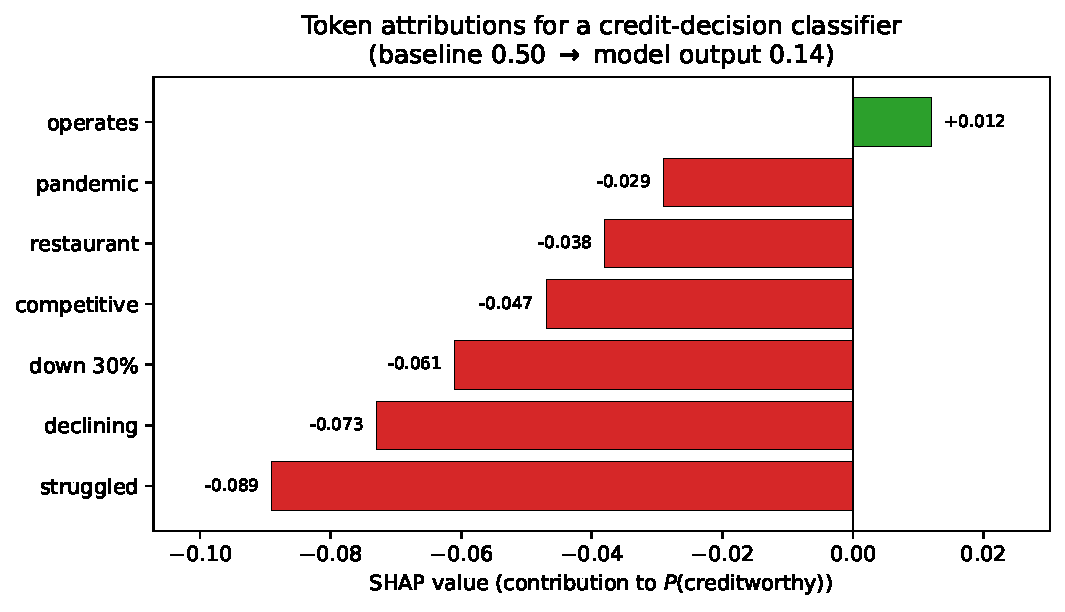
\includegraphics[width=0.74\textwidth]{../../../book/chapters/12-xai-explainability/figures/fig_shap_attribution}
\end{center}
\footnotesize
Token-level SHAP attributions: red (negative) tokens push $P(\text{creditworthy})$
down from the $0.50$ baseline toward $0.14$; ``operates'' adds $+0.012$. Generated
\emph{deterministically} by \texttt{gen\_shap\_attribution.py} from the fixed
example values --- no live model or data.
\end{frame}

% --- Appendix: further reading ---
\begin{frame}[noframenumbering]{Appendix D: Further Reading}
\footnotesize
\begin{itemize}
  \item \textbf{Foundations:} Shapley (1953) axiomatic uniqueness; Lundberg \&
        Lee (2017) unified additive attribution; Lundberg et al.\ (2020) TreeSHAP.
  \item \textbf{LIME:} Ribeiro et al.\ (2016) --- readable, worked text/image/tabular examples.
  \item \textbf{Evaluation:} Doshi-Velez \& Kim (2017) --- vocabulary for human-subject XAI.
  \item \textbf{Counterfactuals:} Wachter et al.\ (2017) --- includes GDPR Art.\ 22 context.
  \item \textbf{Human side:} Miller (2019) --- what users actually want from explanations.
  \item \textbf{Attention debate:} Jain \& Wallace (2019) \emph{vs.}\ Wiegreffe \&
        Pinter (2019); resolution by Jacovi \& Goldberg (2020).
  \item \textbf{Regulation:} EU AI Act (2024); ESMA MiFID II suitability; Fed SR
        11-7; CFA Institute (2025) industry survey; Arrieta et al.\ (2020) full taxonomy.
\end{itemize}

\medskip
\textbf{Within this course:} Credit Risk (calibration, validation prerequisites
for SHAP pipelines); LLM Agents (CoT as planning); Applications \& Future
(fairness / bias, tied to ECOA non-discrimination).
\end{frame}

\end{document}
